\section{Design Challenges}
\label{sec:challenges}

In this paper, we focus on designing systems that sort large datasets as an
instance of the larger problem of building balanced systems.  Here, we discuss
the challenges involved, and outline the key insights underlying our approach.

\subsection{Software Architecture}

Our initial implementation of \tritonsort was designed as a distributed,
two-phase, parallel external merge-sort.  This architecture, which we will call
the Heaper-Merger architecture, is structured as follows.  In the first phase,
Readers read from the input files into buffers, which are sorted by Sorters.
Each sorted buffer is then passed to a Distributor, which splits the buffer
into a sorted chunk per node and sends each chunk to its corresponding node.
Once received, these sorted chunks are heap-sorted by software elements called
Heapers in batches and each resulting sorted batch is written to an
intermediate file on disk.  In the second phase, software elements called
Mergers merge-sort the intermediate files on a given disk into a single sorted
output file.

\begin{figure}
 \centering
 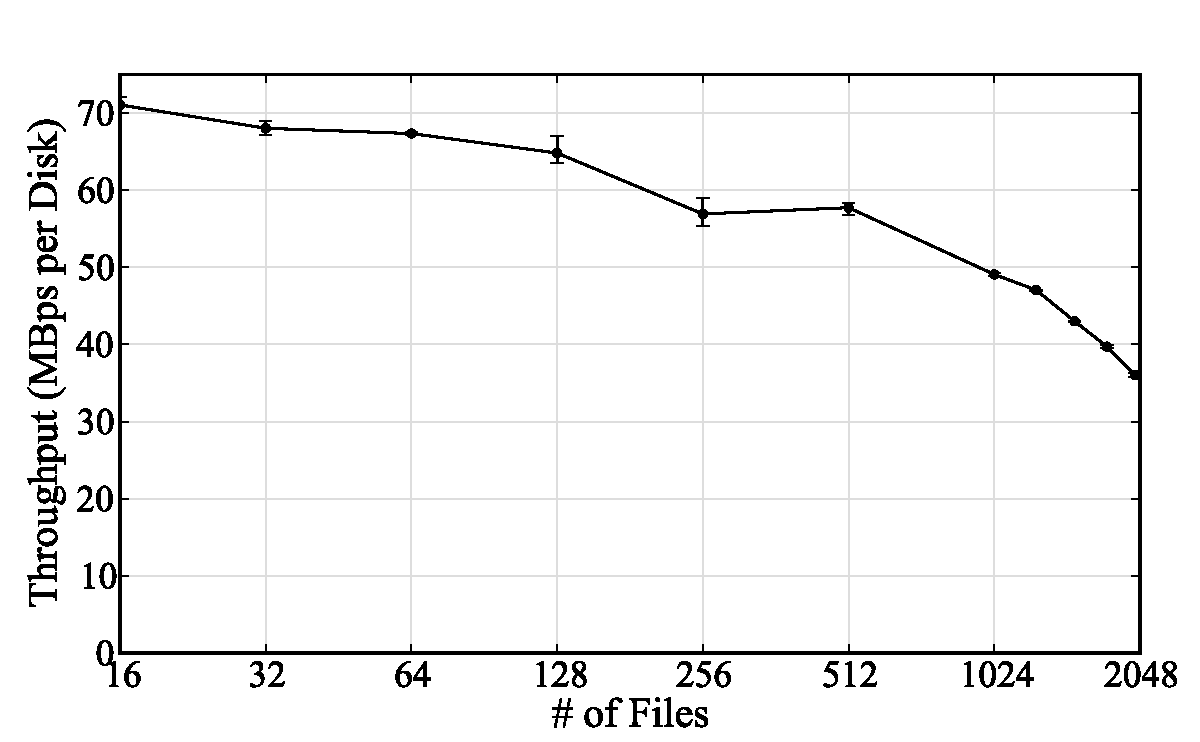
\includegraphics[width=\textwidth]{tritonsort/graphs/mergesortbench.pdf}

 \caption{Performance of a Heaper-Merger sort
   implementation in microbenchmark on a 200GB per disk parallel external merge-sort as a function of the number of files merged per disk.}
 \label{fig:mergesort}
\end{figure}

The problem with the Heaper-Merger architecture is that it does not scale well.
In order to prevent the Heaper in phase one from becoming a bottleneck, the the
sorted runs that the Heaper generates are usually fairly small, on the order of
a few hundred megabytes. As a consequence, the number of intermediate files
that the Merger must merge in phase two grows quickly as the size of the input
data increases. This reduces the amount of data from each intermediate file
that can be buffered at a time by the Merger and requires that the merger fetch
additional data from files much more frequently, causing many additional seeks.

To demonstrate this problem, we implemented a simple Heaper-Merger sort module
in microbenchmark. We chose to sort 200GB per disk in parallel across all the
disks to simulate the system's performance during a 100TB sort. Each disk's
200GB data set is partitioned among an increasingly large number of files. Each
node's memory is divided such that each input file and each output file can be
double-buffered. As shown in Figure~\ref{fig:mergesort}, increasing the number
of files being merged causes throughput to decrease dramatically as the number
of files increases above 1000.

\tritonsort uses an alternative architecture with similar software elements as
above and again involving two phases, as mentioned in
Chapter~\ref{chapter:background}.  We partition the input data into a set of
logical \emph{partitions}; with $D$ physical disks and $L$ logical partitions,
each logical partition corresponds to a contiguous $\frac{1}{L}^{th}$ fraction
of the key space and each physical disk hosts $\frac{L}{D}$ logical partitions.
In the first phase, Readers pass buffers directly to Distributors.  A
Distributor maps the key of every record in its input buffer to its
corresponding logical partition and sends that record over the network to the
machine that hosts this logical partition.  Records for a given logical
partition are buffered in memory and written to disk in large chunks in order
to seek as little as possible.  In the second phase, each logical partition is
read into an in-memory buffer, that buffer is sorted, and the sorted buffer is
written to disk.  This scheme bypasses the seek limits of the earlier
mergesort-based approach.  Also, by appropriately choosing the value of $L$, we
can ensure that logical partitions can be read, sorted and written in parallel
in the second phase.  Since our testbed nodes have 24GB of RAM, to ensure this
condition we set the number of logical partitions per node to 2520 so that each
logical partition contains less than 1GB of records when we sort 100 TB on 52
nodes.  We explain this architecture in more detail in the context of our
implementation in the next section.

% LocalWords:  mergesortbench pdf SSD GraySort Infiniband CPUs SATA Heapers th
% LocalWords:  Distributers LocalWords
